
\documentclass{beamer}

\usepackage{algpseudocode, color, colortbl}

\usepackage{hyperref}
\hypersetup{
    colorlinks=true,
    urlcolor=blue,
}

\usetheme{Montpellier}
\usecolortheme{rose}

% page numbers, from
% https://tex.stackexchange.com/questions/137022/how-to-insert-page-number-in-beamer-navigation-symbols
\expandafter\def\expandafter\insertshorttitle\expandafter{%
  \insertshorttitle\hfill%
  \insertframenumber\,/\,\inserttotalframenumber}

\definecolor{Gray}{gray}{0.8}
\newcolumntype{g}{>{\columncolor{Gray}}c}

\newcommand{\stanza}{ \\~\ }

\title{06. Problem Solving for Algorithm Design}
\subtitle{CPSC 535 $\sim$ Spring 2019}
\author{Kevin A. Wortman}
\institute{ 
\includegraphics[height=2cm]{csuf-logo-cmyk} }
\date{March 4, 2019 \stanza

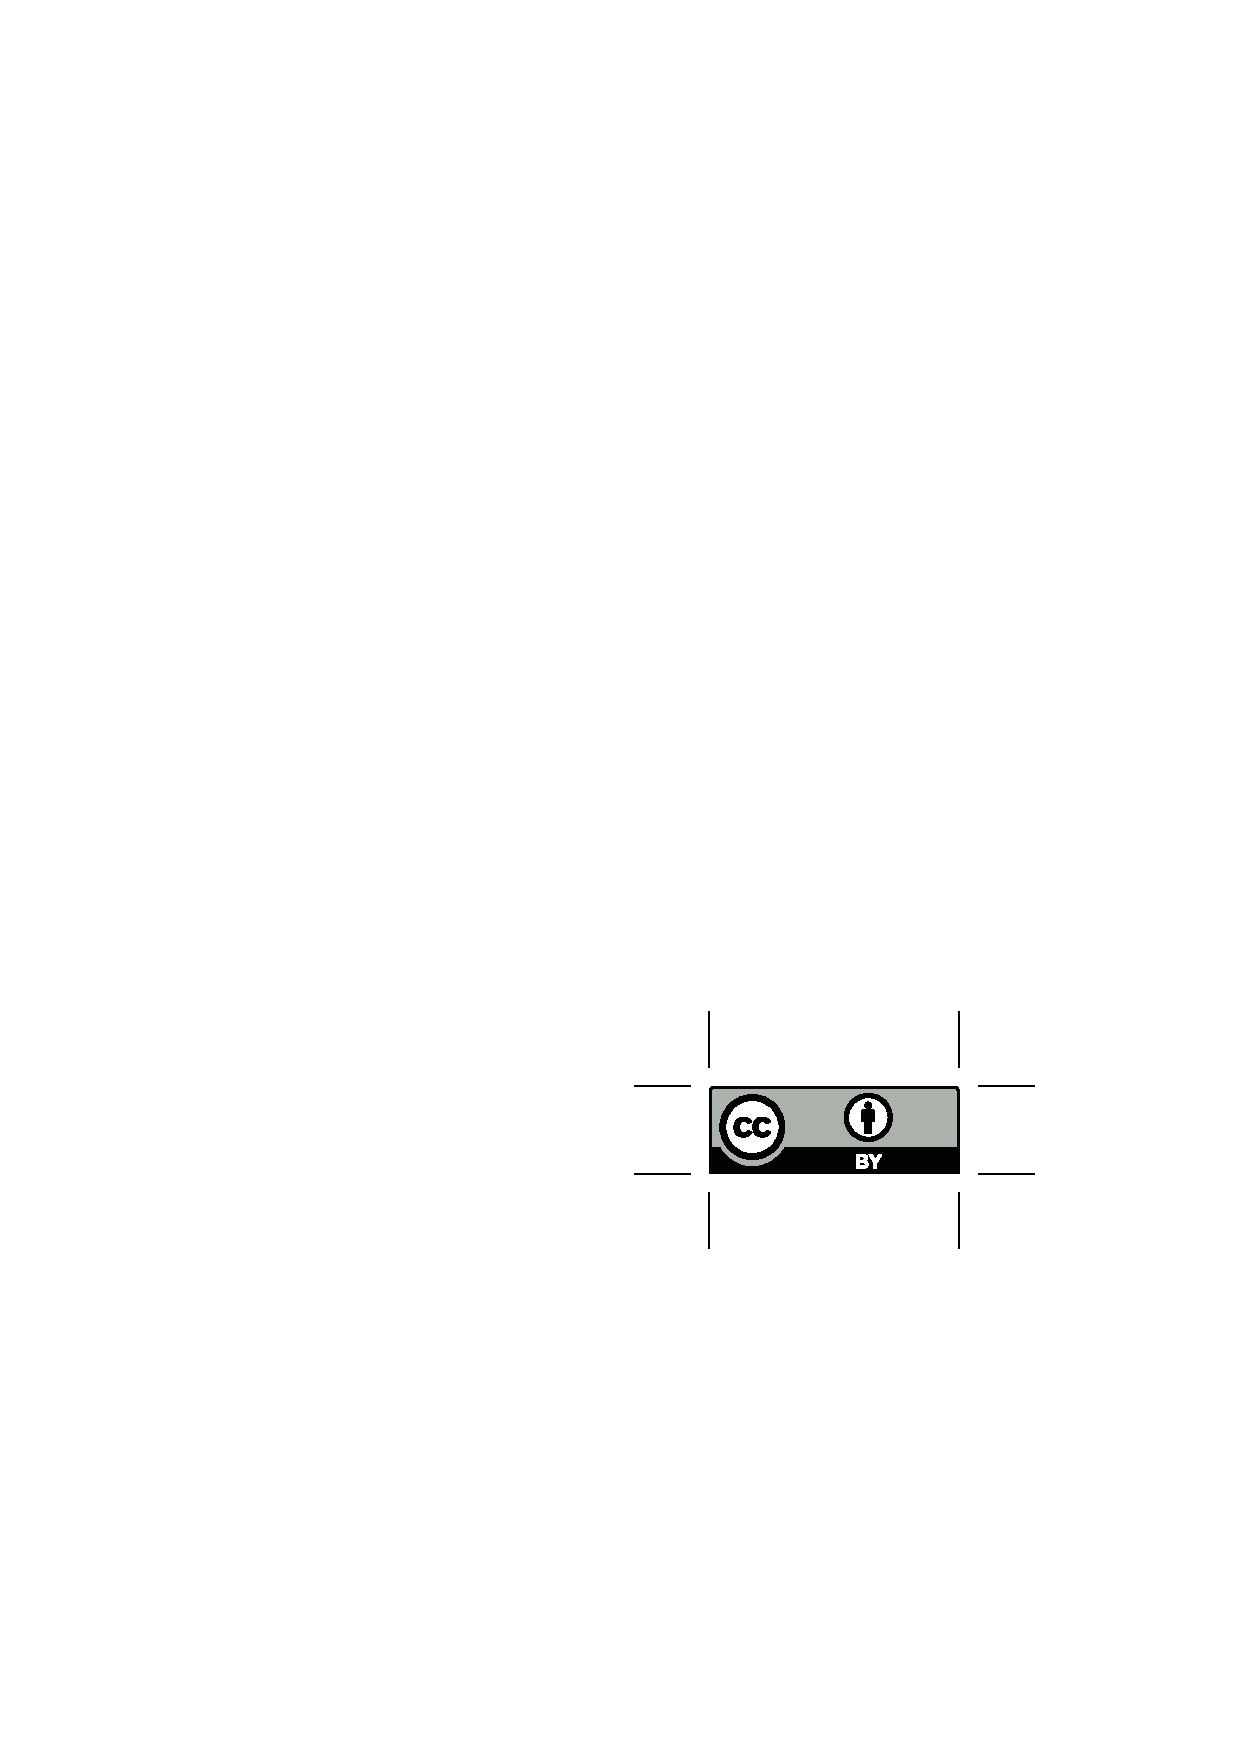
\includegraphics[height=14pt]{by} \\

{\tiny
This work is licensed under a
\href{http://creativecommons.org/licenses/by/4.0/}{Creative Commons Attribution 4.0 International License}.
}}

\begin{document}

\begin{frame}
  \titlepage
\end{frame}

\begin{frame} \frametitle{Overview}
Strategies for designing algorithms in the context of
\begin{itemize}
  \item novel scholarly research
  \item industrial software development \emph{(algorithm engineering)}
  \item technical interviews
  \item class exercises
  \item exam questions
\end{itemize}

Commonalities
\begin{itemize}
  \item partial credit
  \item another person to talk to
\end{itemize}
\end{frame}

\begin{frame} \frametitle{A Checklist}
  \begin{enumerate}
    \item \textbf{Understand} the problem definition
    \item \textbf{Baseline} algorithm for comparison
    \item \textbf{Goal} setting: improve on the baseline how?
    \item \textbf{Design} a more sophisticated algorithm
    \item \textbf{Inspiration} (if necessary) from patterns, bottleneck in the
      baseline algorithm, other algorithms
    \item \textbf{Analyze} your solution; goal met? trade-offs?
  \end{enumerate}
\end{frame}

\begin{frame} \frametitle{1. Understand}
  \begin{itemize}
    \item Read the problem definition (input/output) carefully and critically.
    \item Make sure that you understand the data types involved, constraints on them,
      technical terms, and story of the problem.
      \item Write out a straightforward input and output. Try additional examples
        involving non-obvious solutions.
    \item What are the \emph{corner cases} of input? Can the input be empty?
      When is the solution obvious, and when is it not?
    \item What is a use case for this algorithm in practical software?
    \item Does this problem resemble other problems you know about?
    \item If any of this is unclear, \textbf{ask questions}.
  \end{itemize}
\end{frame}

\begin{frame} \frametitle{Example Problem: Top 25 Words \footnote{Credit: \href{https://www.crcpress.com/Exercises-in-Programming-Style/Lopes/p/book/9781482227376}{Exercises in Programming Style, Christa Lopes}}}
\textbf{input:} a document $D$ (list of $n$ strings) and set
  set $S$ of stop-words (strings) \\
\textbf{output:} a list of pairs
  $T=\{(w, k) : w \in W, w \notin S, \text{ and } k \in \mathbb{N} \}$
  containing the 25 most frequently-occuring words, not including stop-words,
  and the number of times each appears \\
\vspace{12pt}
  Quiz:
  \begin{itemize}
    \item Data types, constraints, of input/output
    \item Example input and output
    \item Corner cases
    \item Use case
    \item Similar to anything familiar?
  \end{itemize}

\end{frame}

\begin{frame} \frametitle{2. Baseline}
Now that you understand the problem, quickly identify at least one algorithm
that solves it.
\begin{itemize}
  \item (research context) literature review: CLRS, Wikipedia, Google Scholar
  \item sketch a \textbf{na\"{i}ve algorithm}: brute force, exhaustive search,
    for loops
  \item What is the efficiency of your baseline algorithm?
  \item Baseline alg. almost always exists
    \begin{itemize}
      \item in our contexts, problems are almost always in $NP$
      \item $\implies$ exponential-time exhaustive search algorithm
    \end{itemize}
  \item In the unlikely event no alg. seems to exist, consider whether the
    problem is provably undecidable.
\end{itemize}
\end{frame}

\begin{frame} \frametitle{Stop after the Baseline?}
Consider: baseline algorithm is a working, but possibly very inefficient, solution to
your problem. \stanza
\begin{itemize}
  \item might be acceptable in S.W.E. if efficiency is low priority
  \item shows technical interviewer that you can communicate and think about
    algorithms
  \item earns partial credit on class assignments
  \item time/labor management
\end{itemize}
\vspace{.5cm}
\emph{Pareto principle (80/20 rule):} in many settings, spending 20\% of
maximum effort achieves 80\% of maximum benefit
\end{frame}

\begin{frame} \frametitle{3. Goal}
What about the baseline do we want to improve?
\begin{itemize}
  \item better \textbf{time efficiency} (most common goal)
  \item better space efficiency
  \item avoid randomization
  \item avoid amortization
  \item extra feature e.g. sort is in-place
  \item simplicity; elegance; easier to implement/understand
  \item better constant factors
\end{itemize}
(non-research contexts): goal may be dictated to you
\end{frame}

\begin{frame} \frametitle{4. Design}
Now, design an algorithm, hopefully achieving your goal. \stanza

Start with verbal discussion; informal sketches; snippets of pseudocode, prose,
equations \stanza

As ideas develop and become more concrete, move to pseudocode. \stanza

Finally write complete, clear pseudocode for the entire algorithm. \stanza

``Devil is in the details:'' resist urge to avoid a tricky part, often that
is the key to meeting your goal. \stanza
\end{frame}

\begin{frame} \frametitle{5. Inspiration}
Step 4. Design...
\begin{enumerate}
  \item \emph{might} come naturally, devise an algorithm effortlessly
  \item \emph{more likely:} not immediately apparent how to proceed; stuck
    at first
\end{enumerate}
\vspace{.5cm}
Case 2 is
\begin{itemize}
  \item more likely
  \item a learned skill
  \item requires practice, effort, experience
  \item point of class exercises
  \item why algorithm design is an in-demand skill
\end{itemize}
\end{frame}

\begin{frame} \frametitle{Sources of Inspiration: algorithm design patterns}
\begin{itemize}
  \item greedy
  \item divide-and-conquer
  \item randomization
  \item reduction to another algorithm (sorting) or data structure (hash table,
    search tree, heap, etc.)
  \item dynamic programming
\end{itemize}
\vspace{.5cm}
Run through the list; can you think of how to use any of these patterns to solve
the problem at hand? \stanza

If a pattern doesn't seem to work, why is that? Might give a hint about what
would work instead.
\end{frame}

\begin{frame} \frametitle{Sources of Inspiration: Identify Bottleck}
Review the analysis of your baseline algorithm (either from the literature,
or what you just devised). \stanza

Identify the dominating term in the efficiency analysis. \stanza

Trace that term backwards to a part of the baseline algorithm; probably a
particular loop or data structure operation. \stanza

How can we do less work there?
\begin{itemize}
  \item preprocessing (ex. maximum subarray)
  \item use an appropriate data structure (ex. heap sort)
  \item reuse work instead of repeating work (ex. Dijkstra's alg.)
  \item dynamic programming
\end{itemize}
\end{frame}

\begin{frame} \frametitle{Sources of Inpiration: Other Algorithms}
One reason we study specific algorithms in detail is to learn about
clever ``tricks'' other designers have used, that we might be able to use in
novel circumstances. \stanza

Examples
\begin{itemize}
  \item define invariants to keep yourself organized (selection sort)
  \item break down problem into simpler phases (heap sort)
  \item use pointers so you can change many paths w/ one assignment;
    redirection (search trees)
  \item use an array instead of pointers (heapsort, open addressing)
  \item master theorem insights to refactor work out of dominating term
    (selection)
  \item when almost all candidate solutions are clearly right/wrong, randomize
    (quicksort, universal hashing)
  \item compute word-at-a-time (hashing, radix sort)
\end{itemize}
\end{frame}

\begin{frame} \frametitle{6. Analyze}
Finally analyze your algorithm. \stanza

Does it meet your goal? (time efficiency, space efficiency, randomization, etc.) \stanza

If yes, obviously done. \stanza

If not,
\begin{itemize}
  \item Is your algorithm still an improvement over your baseline?
  \item Is more effort justified? (Pareto principle.)
  \item If so go back to prior steps.
\end{itemize}
\end{frame}

\end{document}
